% Compiling this file requires that you have AMS-LaTeX 2.0 installed
% as well as the rest of the prerequisites for REVTeX 4.0
%
% See the REVTeX 4 README file
% It also requires running BibTeX. The commands are as follows:
%
%  1)  latex apssamp.tex
%  2)  bibtex apssamp
%  3)  latex apssamp.tex
%  4)  latex apssamp.tex
%
\documentclass[prb,amsmath,amssymb, 10pt]{revtex4}
%\documentclass[preprint,showpacs,showkeys,preprintnumbers,amsmath,amssymb]{revtex4}

% Some other (several out of many) possibilities
%\documentclass[preprint,aps]{revtex4}
%\documentclass[aps, two column, amsmath,amssymb,floatfix]{revtex4}
%\documentclass[showkeys,showpacs,amsmath,amssymb,onecolumn,superscriptaddress,prl]{revtex4-1}% Physical Review B  
% \documentclass[aps,prl,reprint,showpacs,floatfix,superscriptaddress, onecolumn]{revtex4-2}

\usepackage{amsmath,amsthm,amssymb}
\usepackage{graphicx}% Include figure files
\usepackage{dcolumn}% Align table columns on decimal point
\usepackage{bm}% bold math
\usepackage{color}
\usepackage{epsfig}
\usepackage{multirow}
\usepackage{mathrsfs}
\usepackage{hyperref}
\usepackage{cleveref}
\usepackage{epstopdf}
\usepackage{subcaption}
\usepackage{autobreak}
\usepackage{tikz}
\usepackage{svg}
\usepackage{placeins}

%Macros for mathematical notations

\newcommand{\V}[1]{\boldsymbol{#1}} %# vector
\newcommand{\M}[1]{\boldsymbol{#1}} %# matrix
\newcommand{\Set}[1]{\mathbb{#1}} %# set
\newcommand{\D}[1]{\Delta#1} %# \D{t} for time step size
\renewcommand{\d}[1]{\delta#1} %# \d{t} for small increment
\newcommand{\norm}[1]{\left\Vert #1\right\Vert } % norm
\newcommand{\abs}[1]{\left|#1\right|} %abs

\newcommand{\grad}{\M{\nabla}} %gradient
\newcommand{\av}[1]{\left\langle #1\right\rangle } %take average

\newcommand{\sM}[1]{\M{\mathcal{#1}}} %matrix in mathcal font
\newcommand{\dprime}{\prime\prime} % double prime
%\global\long\def\i{\iota}
%\renewcommand{\i}{\iota} %i for imaginary unit
%\renewcommand{\i}{\mathsf i} %i for imaginary unit
\newcommand{\follows}{\quad\Rightarrow\quad} %=>
\newcommand{\eqd}{\overset{d}{=}} %=^d
\newcommand{\spe}[1]{\mathscr{#1}}  %important quantities in mathscr font
\newcommand{\eps}{\epsilon}
\newcommand{\bra}[1]{\left\langle #1 \right|}
\newcommand{\ket}[1]{\left| #1 \right\rangle}
\newcommand{\braket}[2]{\left\langle #1 \middle| #2 \right\rangle}
\newcommand{\bracket}[3]{\left\langle #1 \middle| #2 \middle| #3 \right\rangle}

\newtheorem{theorem}{Theorem}[section]
\newtheorem{lemma}[theorem]{Lemma}
\newtheorem{definition}[theorem]{Definition}



\begin{document}
\preprint{Preprint}

\title{Orbital Density Across the Interface}
\author{Xuanzhao Gao}
% \date{}

\maketitle

\section{Basic Idea}

In this note, we consider the case in which the orbital density crosses the box, introducing a discontinuity across the boundary.
A simple schematic of this case is shown in Fig.~\ref{fig:orbital_cross_interface}, where the density~$\rho(x)$ is separated into two parts, $\rho_1$ and $\rho_2$, by the interface. The permittivities on the two sides of the interface are~$\epsilon_1$ and~$\epsilon_2$, respectively.

\begin{figure}[htbp]
    \centering
    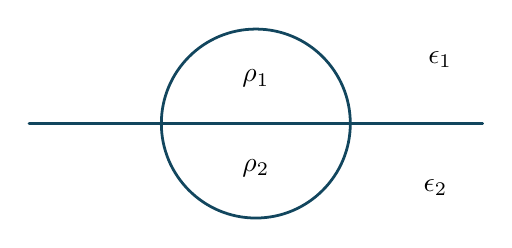
\begin{tikzpicture}[scale=0.6, line join=round, line cap=round]
        \definecolor{interfacecolor}{RGB}{18,70,94}

        \draw[interfacecolor, line width=1pt] (-4.8,0) -- (4.8,0);
        \draw[interfacecolor, line width=1pt] (0,0) circle (2.0);

        \node at (0,0.95) {$\rho_1$};
        \node at (0,-0.95) {$\rho_2$};
        \node at (3.9,1.35) {$\epsilon_1$};
        \node at (3.8,-1.35) {$\epsilon_2$};
    \end{tikzpicture}
    \caption{Schematic of an orbital density crossing a planar dielectric interface.}
    \label{fig:orbital_cross_interface}
\end{figure}

Recall that the incident potential~$u_{\text{inc}}(x)$ should satisfy
\begin{equation}
    \epsilon_i \nabla^2 u_{\text{inc}}(x) = -\rho(x),~x \in \Omega_i,
\end{equation}
and it can be expressed as follows:
\begin{equation}
    u_{\text{inc}}(x) = \sum_{i} \int_{\Omega_i} G(x,y) \frac{\rho_i(y)}{\epsilon_i} dy,
\end{equation}
where $G(x, y)$ is the free-space Green's function.
Thus, we define the ``screened charge density'', and rewrite the incident potential in terms of the screened charge density:
\begin{equation}
    \tilde{\rho}(y) = \frac{\rho_i(y)}{\epsilon_i},~y \in \Omega_i, \quad u_{\text{inc}}(x) = \sum_{i} \int_{\Omega} G(x,y) \tilde{\rho}_i(y) dy,
\end{equation}
and the single layer surface charge density $\sigma(x)$ should again satisfy
\begin{equation}\label{eq:sl_equation}
    \left( \frac{1}{2} \frac{\epsilon_i + \epsilon_j}{\epsilon_i - \epsilon_j} + D^T \right) \sigma(x) = - \partial_{\mathbf{n}} u_{\text{inc}}(x),~x \in \partial \Omega_i \cap \partial \Omega_j,
\end{equation}
which is a Fredholm integral equation of the second kind~\cite{greengard1994numerical}.

\begin{figure}[htbp]
    \centering
    \includesvg[width=0.85\textwidth]{../codes/volume_source/figs/screened_gauss_ft.svg}
    \caption{Screened Gaussian functions and their Fourier transforms.}
    \label{fig:screened_gauss_ft}
\end{figure}

Notice that~$\tilde{\rho}(y)$ is discontinuous across the interface, which makes its Fourier transform decay slowly, as shown by the blue curve in Fig.~\ref{fig:screened_gauss_ft}. Therefore, it is not suitable for our TKM-Fourier solver.
Considering the physical model of the system, the dielectric permittivity should not change sharply, especially on the atomic scale. We therefore propose replacing the screening function with a smooth function that transitions continuously across the interface, such as the $\text{erf}(\cdot)$ function.
In this way, we can obtain a screened charge density that is continuous across the interface, and its Fourier transform decays rapidly, also shown in Fig.~\ref{fig:screened_gauss_ft}.
This also allows us to tune the bandwidth of the screening function to match the experimental or full ab initio results of pairwise interactions.

For an interface, there are two different ways to create a smooth transition of the dielectric permittivity.
The first is to mix the permittivity directly:
\begin{equation}
    \tilde{\epsilon}(x) = \epsilon_1 P(x) + \epsilon_2 (1 - P(x)),
\end{equation}
where $P(x)$ is a smooth function that transitions from 1 to 0 across the interface, such as the $\text{erf}(\cdot)$ function.
This approach seems more reasonable in a physical sense.
Another choice is to mix the inverse permittivity, which gives a smoother transition of the effective screened charge density:
\begin{equation}
    \tilde{\epsilon}(x) = \frac{1}{\frac{P(x)}{\epsilon_1} + \frac{1 - P(x)}{\epsilon_2}}.
\end{equation}

Thus, we propose a combination of two different models: for the calculation of the incident potential, we assume that the dielectric permittivity changes smoothly across the interface; for the calculation of the single-layer potential, we use the original model with a sharp interface for ease of calculation.
This way, we can still use the TKM-Fourier solver to compute the incident potential, and then solve the single layer potential using the original model with a sharp interface.
We can rewrite the equations as follows:
\begin{align}
    u_{\text{inc}}^\prime(x) &= \int_{\Omega} G(x,y) \tilde{\rho^\prime}(y) dy, \\
    \left( \frac{1}{2} \frac{\epsilon_i + \epsilon_j}{\epsilon_i - \epsilon_j} + D^T \right) \sigma(x) &= - \partial_{\mathbf{n}} u_{\text{inc}}^\prime(x),~x \in \partial \Omega_i \cap \partial \Omega_j,
\end{align}
and the scattered potential can be computed as
\begin{equation}
    u_{\text{scat}}(x) = \int_{\partial \Omega} G(x,y) \sigma(y) dy.
\end{equation}

\section{Numerical Results}

In this section, we present some preliminary numerical results for the proposed method.
We first examine the decay of the Fourier transform of the screened orbital density in the $k_z$ direction, as shown in Fig.~\ref{fig:graphene_screened_density_kz_decay}.
The original screened density is discontinuous across the interface, and its Fourier transform decays slowly even with upsampling.
The smoothed screened density is continuous across the interface, and its Fourier transform decays rapidly, which is suitable for our TKM-Fourier solver.


\begin{figure}[htbp]
    \centering
    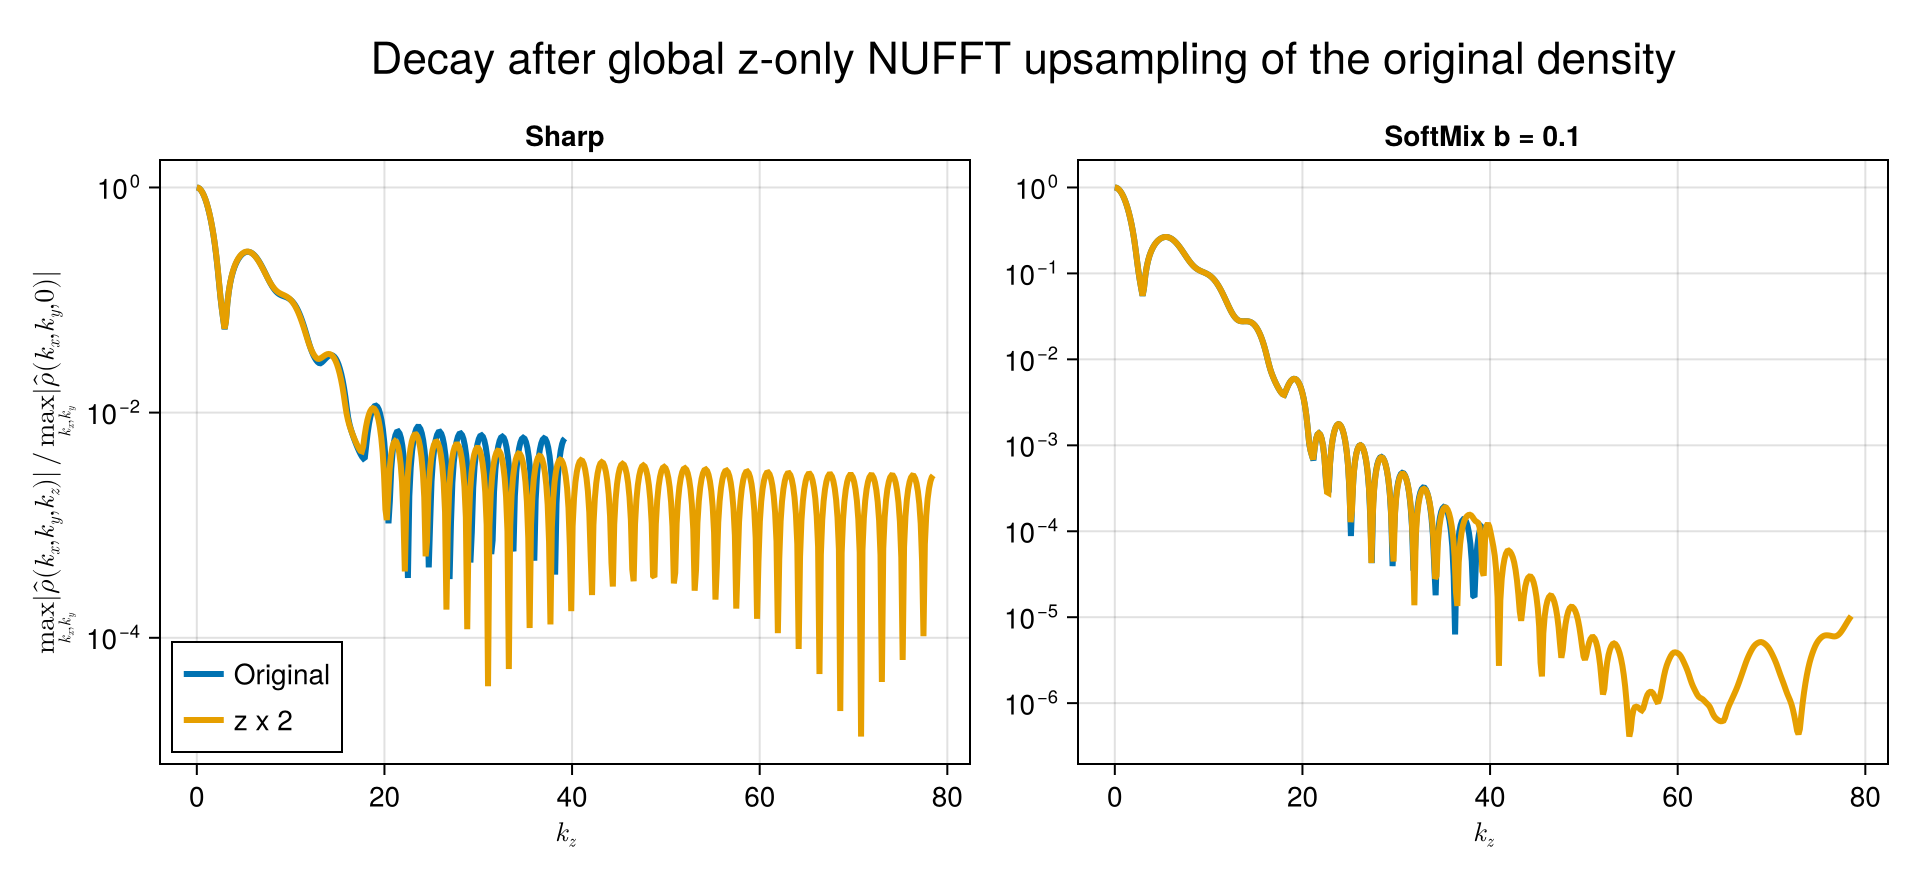
\includegraphics[width=0.6\textwidth]{../codes/graphene/figs/screened_density_kz_decay_z_upsampled.png}
    \caption{Screened orbital functions with upsampling in $z$ and their Fourier transforms.}
    \label{fig:graphene_screened_density_kz_decay}
\end{figure}

We then consider a full solve for the graphene system, using an effective dielectric model with $L_x = L_y = 90~\text{\AA}$, $L_z = 2.8~\text{\AA}$, and $\epsilon_r = 2.4$, and evaluate $U_{00}$, $U_{01}$, $U_{02}$, and $U_{03}$ as defined in Ref.~\cite{PhysRevLett.106.236805}.
The results are shown in Fig.~\ref{fig:screened_hubbard_vs_crpa}, where we compare the screened Hubbard model with the constrained RPA results from Ref.~\cite{PhysRevLett.106.236805}. The two methods show good agreement for small screening bandwidths.

\begin{figure}[htbp]
    \centering
    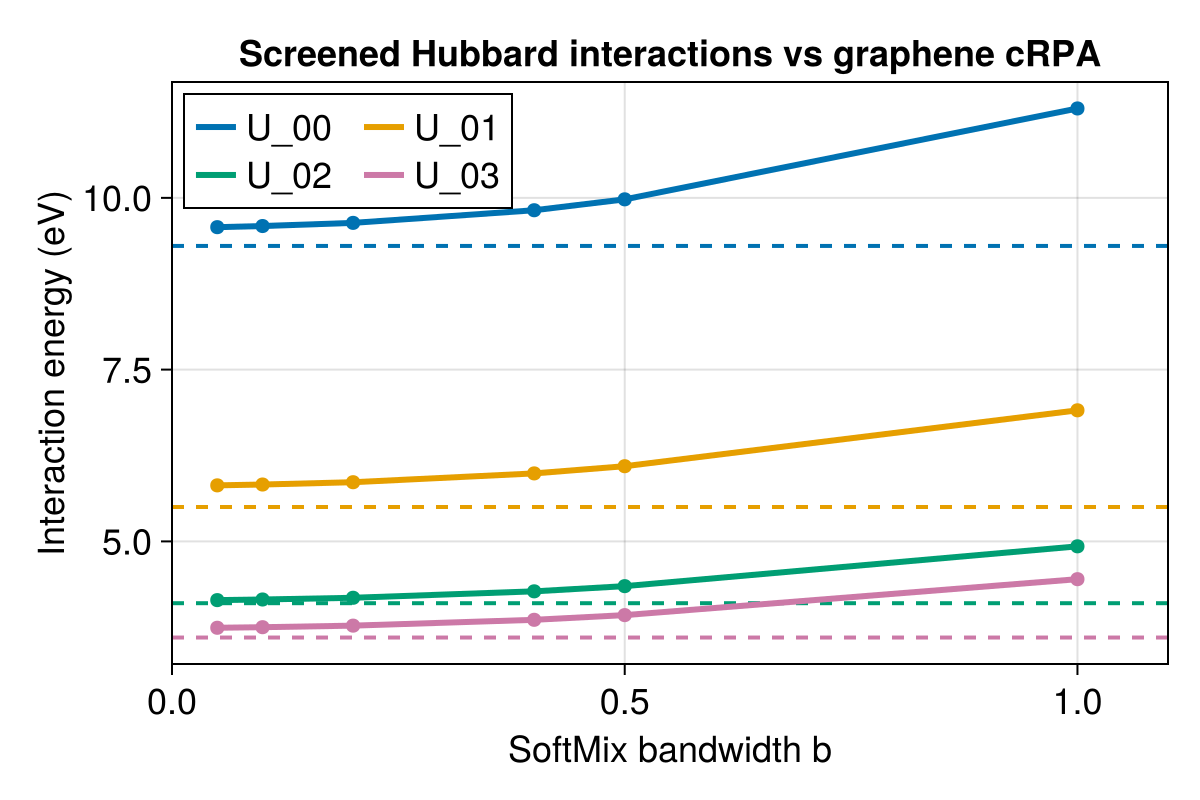
\includegraphics[width=0.5\textwidth]{../codes/graphene/figs/screened_hubbard_vs_crpa.png}
    \caption{Comparison of the screened Hubbard and constrained RPA results. The dashed lines denote the constrained RPA data from Ref.~\cite{PhysRevLett.106.236805}.}
    \label{fig:screened_hubbard_vs_crpa}
\end{figure}

The current code is also ready to solve systems with multiple dielectric boxes, as shown in Fig.~\ref{fig:multiple_boxes}. In this example, the orbital density is located in the slab at the top, and the interface is discretized into panels with refinement near the edges, corners, and orbital density.

\begin{figure}[htbp]
    \centering
    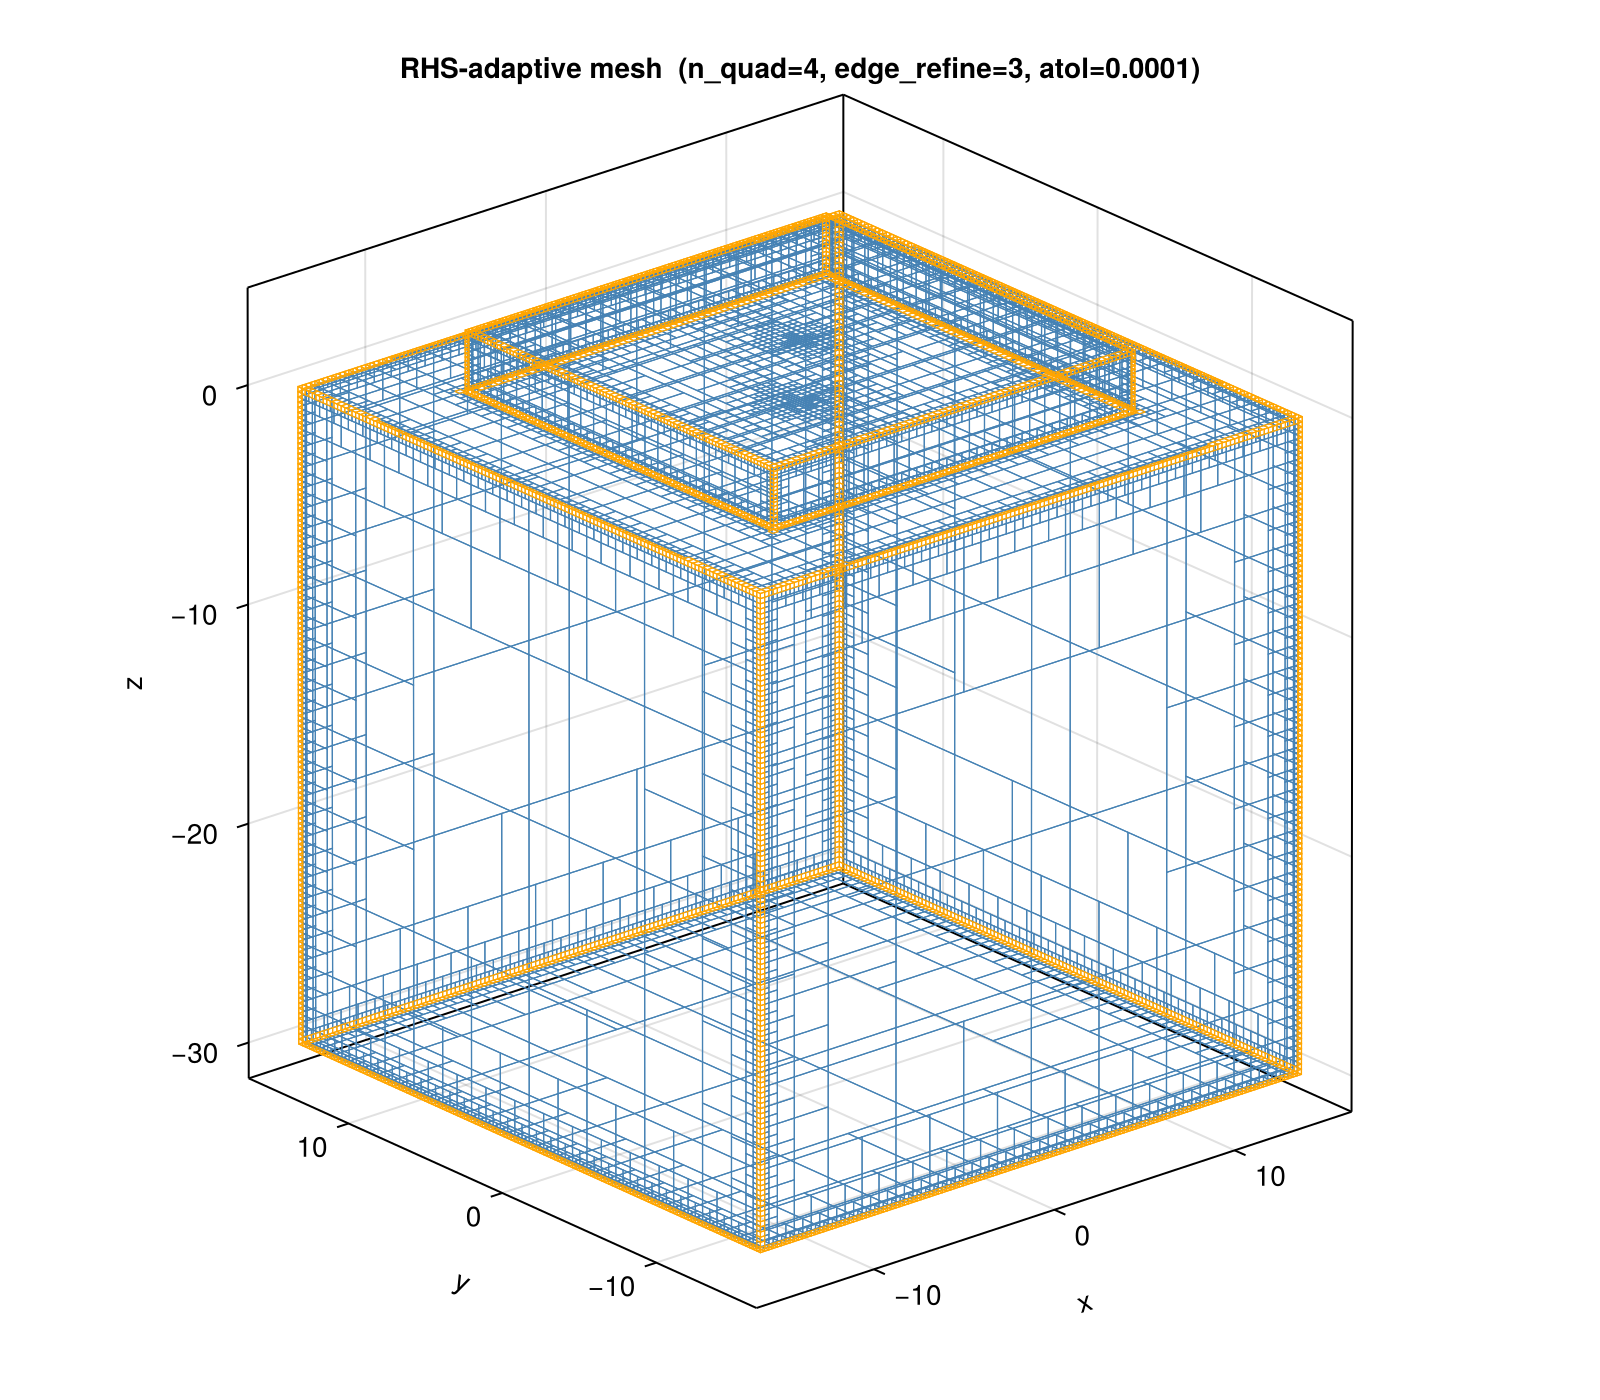
\includegraphics[width=0.6\textwidth]{../codes/multibox3d_convergence/figs/graphene_slab_rhs_mesh.png}
    \caption{Discretized boundary for a system with multiple dielectric boxes. The yellow boxes are edge or corner panels.}
    \label{fig:multiple_boxes}
\end{figure}

% \bibliographystyle{apsrev}
\bibliography{ref}

\end{document}